% SPDX-License-Identifier: PMPL-1.0-or-later
% SPDX-FileCopyrightText: 2026 Jonathan D.A. Jewell
%
% arcvix-code-as-matter.tex — Code as Matter: The Materiality of Linear Types
% This is the second Ephapax paper, distinct from the dyadic language design paper.
% It covers the philosophical/formal insight connecting linear types to physical matter.

\documentclass[11pt,a4paper]{article}

% --- Packages ---
\usepackage[utf8]{inputenc}
\usepackage[T1]{fontenc}
\usepackage{lmodern}
\usepackage{amsmath,amssymb,amsthm}
\usepackage{mathtools}
\usepackage{stmaryrd}
\usepackage{proof}
\usepackage{hyperref}
\usepackage[margin=2.5cm]{geometry}
\usepackage{enumitem}
\usepackage{booktabs}
\usepackage{graphicx}
\usepackage{xcolor}
\usepackage{listings}
\usepackage{tikz}
\usetikzlibrary{arrows.meta,positioning,shapes.geometric,calc}
\usepackage{epigraph}
\usepackage{microtype}
\usepackage{natbib}
\bibliographystyle{plainnat}

% --- Theorem environments ---
\newtheorem{theorem}{Theorem}[section]
\newtheorem{lemma}[theorem]{Lemma}
\newtheorem{proposition}[theorem]{Proposition}
\newtheorem{corollary}[theorem]{Corollary}
\newtheorem{definition}[theorem]{Definition}
\newtheorem{example}[theorem]{Example}
\newtheorem{remark}[theorem]{Remark}
\newtheorem{principle}{Principle}

% --- Listings for Ephapax ---
\lstdefinelanguage{Ephapax}{
  keywords={let, fn, in, region, copy, move, drop, consume, match, with, if, then, else, return, type, struct, enum},
  keywords=[2]{let!},
  keywordstyle=\bfseries\color{blue!70!black},
  keywordstyle=[2]\bfseries\color{red!70!black},
  comment=[l]{//},
  commentstyle=\itshape\color{green!50!black},
  stringstyle=\color{orange!80!black},
  string=[b]",
  basicstyle=\ttfamily\small,
  showstringspaces=false,
  tabsize=4,
  breaklines=true,
  literate={->}{$\rightarrow$}{2} {@}{@}{1},
}

\lstset{
  language=Ephapax,
  frame=single,
  framerule=0.4pt,
  rulecolor=\color{gray!50},
  backgroundcolor=\color{gray!5},
  xleftmargin=1em,
  xrightmargin=1em,
}

% --- Macros ---
\newcommand{\Linear}{\textsf{Lin}}
\newcommand{\Affine}{\textsf{Aff}}
\newcommand{\Unres}{\textsf{Un}}
\newcommand{\ephapax}{\textsc{Ephapax}}
\newcommand{\letbang}{\texttt{let!}}
\newcommand{\letkw}{\texttt{let}}
\newcommand{\consume}{\triangleright}
\newcommand{\tensor}{\otimes}
\newcommand{\lolli}{\multimap}
\newcommand{\bang}{!}

% --- Title ---
\title{%
  \textbf{Code as Matter: The Materiality of Linear Types \\
  and the Refinement Journey from Affine Drafting \\
  to Linear Commitment}%
}

\author{%
  Jonathan D.A. Jewell \\
  \texttt{j.d.a.jewell@open.ac.uk} \\
  \medskip
  \small The Open University
}

\date{March 2026}

\begin{document}

\maketitle

% ============================================================================
% ABSTRACT
% ============================================================================
\begin{abstract}
We propose that linear types are not merely a programming language feature
but a formal model of physical materiality itself. A linear binding---one that
must be consumed exactly once, can be neither duplicated nor silently
discarded---possesses the ontological status of \emph{matter}: it obeys
conservation laws, has identity, and participates in transformations rather
than copies. We develop this \emph{materiality thesis} through a systematic
correspondence between substructural type theory and conservation principles
in physics, arguing that unrestricted computation, far from being the
natural default, is the anomalous special case requiring justification.

We formalise a \emph{refinement journey} from affine types (the drafting
space, where resources may be dropped but not duplicated) to linear types
(the commitment space, where every resource must be accounted for), and show
that this journey mirrors the physical transition from model to reality, from
blueprint to built structure. This framework is instantiated concretely in
\ephapax{}, a dyadic language where \letkw{} introduces affine bindings and
\letbang{} introduces linear bindings, making the refinement journey a
first-class syntactic and semantic distinction.

We connect this perspective to Girard's linear logic, Landauer's principle
on the thermodynamic cost of information erasure, Abramsky's computational
interpretations of linear logic, and recent work on reversible computation.
The result is a philosophical framework in which the compiler is reconceived
as a conservation-law enforcement engine, garbage collection is revealed as
the fiction that matter can be wished away, and the ``restriction'' of
linearity is unmasked as fidelity to physical reality.
\end{abstract}

\bigskip

\noindent\textbf{Keywords:} linear types, affine types, substructural logic,
conservation laws, materiality, resource semantics, Landauer's principle,
linear logic, programming language philosophy

\newpage
\tableofcontents
\newpage

% ============================================================================
% 1. INTRODUCTION
% ============================================================================
\section{Introduction}
\label{sec:intro}

\epigraph{%
  ``Information is physical.''
}{Rolf Landauer, 1991}

\noindent
What if we took the physics of computation literally?

Not as metaphor, not as analogy, but as ontological claim: that the
values manipulated by a program have the status of \emph{physical
matter}, and that the type system is not a bookkeeping convenience but
a system of \emph{conservation laws} governing the creation,
transformation, and destruction of that matter.

This paper argues that linear types---the discipline in which every
value must be consumed exactly once---provide precisely such a
physics of computation. Under this reading, a linear binding is not a
``restricted'' version of an ordinary variable. It is the \emph{faithful}
model. It is the ordinary, unrestricted variable that is the
idealisation, the fiction, the approximation that works only because
we have hidden the costs of copying and discarding behind layers of
runtime machinery.

The claim has three parts:

\begin{enumerate}[label=(\roman*)]
\item \textbf{The Materiality Thesis.} A linear value has the
  ontological status of a physical object. It cannot be duplicated
  (conservation of mass), cannot be silently destroyed (conservation
  of energy in transformation), and must participate in exactly one
  transformation event (an event happens once).

\item \textbf{The Refinement Journey.} There is a \emph{directed}
  path from affine types to linear types, corresponding to the
  transition from approximate model to precise reality. Affine
  bindings are the drafting space---sketches that can be abandoned.
  Linear bindings are the commitment space---built structures where
  every beam must bear load.

\item \textbf{The Inversion.} The conventional view that unrestricted
  types are ``normal'' and linear types are ``restricted'' is exactly
  backwards. Linearity is the natural condition; unrestriction is the
  expensive, energy-consuming, entropy-producing anomaly.
\end{enumerate}

We develop these claims formally in the setting of substructural type
theory, connect them to thermodynamics through Landauer's principle,
and instantiate them concretely in the design of \ephapax{}, a
language where the refinement journey from affine drafting to linear
commitment is a first-class syntactic and semantic operation.

The paper is intended to be read in the spirit of Wadler's
``Propositions as Types'' \citep{wadler2015propositions}---not as a
technical contribution in isolation, but as an argument for a
\emph{way of seeing} that connects seemingly distant domains and
reveals structure that was always there.


% ============================================================================
% 2. THE MATERIALITY THESIS
% ============================================================================
\section{The Materiality Thesis}
\label{sec:materiality}

\subsection{Linear Values as Physical Objects}

Consider a physical object---say, a brick. A brick has the following
properties:

\begin{enumerate}[label=(\alph*)]
\item \textbf{Identity.} This brick is \emph{this} brick, not a
  representative of the class of bricks. It occupies a specific
  location, has a specific history, and bears specific marks.

\item \textbf{Non-duplicability.} You cannot copy a brick. You can
  manufacture another brick, but that is a \emph{different} brick,
  requiring raw materials and energy. The copy is not free; it is a
  new act of creation.

\item \textbf{Non-destructibility without transformation.} You cannot
  make a brick vanish. You can crush it, dissolve it, heat it until
  it changes state---but each of these is a \emph{transformation},
  not an annihilation. The matter persists in some form.

\item \textbf{Single-use in context.} A brick placed in a wall is
  \emph{consumed} by that wall. It cannot simultaneously be placed
  in a second wall. Its participation in one structure precludes its
  participation in another (without first removing it---a
  transformation).
\end{enumerate}

Now consider a linear binding in a type system with linear types.
A value bound linearly must be used exactly once. It cannot be
duplicated (no contraction). It cannot be silently discarded (no
weakening). It has identity (it is \emph{this} binding in \emph{this}
scope, not an interchangeable reference to an abstract value).

\begin{principle}[Materiality Principle]
A linear binding has the ontological status of a physical object. The
structural rules it lacks---contraction and weakening---correspond to
conservation laws that physical matter obeys.
\end{principle}

This is not analogy. We claim it is \emph{homomorphism}: the same
abstract structure governs both domains.

\subsection{The Correspondence Table}

Table~\ref{tab:correspondence} makes the correspondence explicit.

\begin{table}[ht]
\centering
\begin{tabular}{@{}lll@{}}
\toprule
\textbf{Physical Law} & \textbf{Type-Theoretic Rule} & \textbf{Meaning} \\
\midrule
Conservation of mass & No contraction & Values cannot be duplicated \\
Conservation of energy & No weakening & Values cannot be silently discarded \\
Identity of indiscernibles & Binding identity & This value, not a representative \\
Single event occurrence & Exactly-once consumption & Used in one context only \\
Transformation, not annihilation & Explicit destructors & Disposal is a visible act \\
Entropy increase & Resource usage ordering & Transformations are irreversible \\
\bottomrule
\end{tabular}
\caption{Correspondence between physical conservation laws and the
  structural discipline of linear types.}
\label{tab:correspondence}
\end{table}

\subsection{What Duplication Really Costs}

In the physical world, copying requires energy. To duplicate a
document, you need paper, ink, and the mechanical energy of a
printer. To copy a biological organism, you need the full metabolic
machinery of cell division. To copy a quantum state, you cannot do
it at all---the no-cloning theorem is a fundamental law of physics
\citep{wootters1982nocloning}.

In conventional programming, duplication appears free. You assign a
variable, and now two names refer to the same value---or, with value
semantics, two independent copies exist with no visible cost. But
this appearance is sustained by invisible machinery: memory
allocation, cache coherence protocols, garbage collection. The cost
is real; it is merely hidden.

Linear types make the cost visible. In a linear type system,
duplication requires an explicit \texttt{copy} operation, which the
type system tracks. This is not a restriction layered on top of a
naturally free operation. It is the \emph{removal of a lie}---the lie
that copying is free.

\begin{remark}
The no-cloning theorem of quantum mechanics \citep{wootters1982nocloning}
can be read as a type-theoretic statement: quantum states are linear.
The universe's fundamental substrate already uses linear types. Classical
computation's ability to copy is not a more general capability---it is a
\emph{lossy projection} of quantum reality onto a simplified model.
\end{remark}


% ============================================================================
% 3. CONSERVATION LAWS IN TYPE SYSTEMS
% ============================================================================
\section{Conservation Laws in Type Systems}
\label{sec:conservation}

\subsection{The Substructural Hierarchy}

Substructural type systems are classified by which structural rules
they admit \citep{walker2005substructural}. The standard hierarchy is:

\begin{definition}[Structural Rules]
Given a typing context $\Gamma$, the \emph{structural rules} are:
\begin{itemize}
\item \textbf{Exchange:} $\Gamma, x : A, y : B \vdash e : C
  \implies \Gamma, y : B, x : A \vdash e : C$
\item \textbf{Weakening:} $\Gamma \vdash e : C \implies
  \Gamma, x : A \vdash e : C$
\item \textbf{Contraction:} $\Gamma, x : A, y : A \vdash e : C
  \implies \Gamma, z : A \vdash e[z/x, z/y] : C$
\end{itemize}
\end{definition}

The hierarchy of substructural systems is then:

\begin{center}
\begin{tabular}{@{}lccc@{}}
\toprule
\textbf{System} & \textbf{Exchange} & \textbf{Weakening} & \textbf{Contraction} \\
\midrule
Unrestricted & \checkmark & \checkmark & \checkmark \\
Affine       & \checkmark & \checkmark & $\times$ \\
Relevant     & \checkmark & $\times$   & \checkmark \\
Linear       & \checkmark & $\times$   & $\times$ \\
Ordered      & $\times$   & $\times$   & $\times$ \\
\bottomrule
\end{tabular}
\end{center}

\subsection{Conservation Laws as Absent Structural Rules}

We now interpret each absent structural rule as a conservation law.

\paragraph{No Contraction = Conservation of Mass.}
If a value cannot be duplicated, then the total ``mass'' of values in
the system is conserved. Each value exists in exactly one location in
the typing context. Creating a second reference requires an explicit
act of creation---a \texttt{copy} operation that the type system
tracks, just as physics tracks the energy expenditure of duplicating
matter.

Formally, in a linear context $\Gamma$, if $x : A \in \Gamma$, then
any derivation $\Gamma \vdash e : B$ uses $x$ at most once (in the
affine case) or exactly once (in the linear case). There is no rule
that transforms one occurrence of $x : A$ into two.

\paragraph{No Weakening = Conservation of Energy.}
If a value cannot be silently discarded, then every value must
participate in some transformation. In physics, energy is never
destroyed---it is transformed from one form to another. Similarly, a
linear value must be \emph{consumed} by some operation. The
consumption might produce new values (as burning wood produces heat
and ash), but the original value does not simply vanish.

The prohibition on weakening means that if $x : A \in \Gamma$ and
$\Gamma \vdash e : B$, then $x$ must appear in $e$. Every resource
in scope must be accounted for.

\paragraph{Exchange Preserved = Space is Homogeneous.}
We retain the exchange rule in both the affine and linear fragments.
This corresponds to the physical principle that the laws of physics
do not depend on the ordering of objects---space is homogeneous. The
order in which resources appear in the context does not affect the
computation. (Ordered types, which drop exchange, correspond to
spatially structured systems where position matters, such as stacks
or queues.)

\subsection{The Conservation Equation}

We can state the conservation principle formally:

\begin{theorem}[Resource Conservation]
\label{thm:conservation}
In a linear type system, let $|\Gamma|$ denote the multiset of types
in context $\Gamma$. If $\Gamma \vdash e : A$, then:
\[
  |\Gamma| = |\Delta_1| \uplus |\Delta_2| \uplus \cdots \uplus |\Delta_n| \uplus \{A\}
\]
where each $\Delta_i$ is consumed by a subexpression of $e$, and
$\uplus$ denotes multiset union. No type in $|\Gamma|$ is lost or
duplicated.
\end{theorem}

\begin{proof}[Proof sketch]
By structural induction on the derivation of $\Gamma \vdash e : A$.
Each rule in linear logic splits the context exactly, with no
residual unused assumptions. The multiplicative rules ($\tensor$,
$\lolli$) partition the context between premises; the additive rules
($\&$, $\oplus$) require both premises to use the same context.
In no case is a hypothesis duplicated or discarded.
\end{proof}

This is the type-theoretic analogue of the conservation equation in
physics:
\[
  \sum_i m_i^{\text{in}} = \sum_j m_j^{\text{out}}
\]
The ``mass'' going in equals the ``mass'' coming out.


% ============================================================================
% 4. THE REFINEMENT JOURNEY
% ============================================================================
\section{The Refinement Journey}
\label{sec:refinement}

\subsection{Affine as Drafting, Linear as Commitment}

The central design insight of \ephapax{} is that affine and linear types
are not parallel alternatives but \emph{stages on a directed journey}.

\begin{definition}[The Refinement Ordering]
Define a partial order on type modalities:
\[
  \Unres \sqsubseteq \Affine \sqsubseteq \Linear
\]
where $\sqsubseteq$ is read ``is refined by.'' Moving right in this
ordering increases the fidelity of the model: from unrestricted
(anything goes) through affine (no duplication, but dropping allowed)
to linear (no duplication, no dropping---full conservation).
\end{definition}

This ordering has a natural interpretation:

\begin{center}
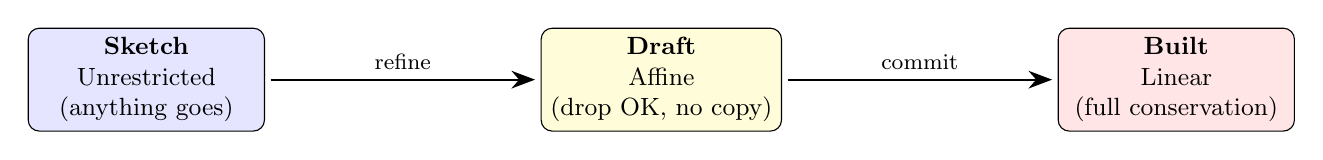
\begin{tikzpicture}[
  node distance=3.5cm,
  stage/.style={draw, rounded corners, minimum width=3cm, minimum height=1.2cm,
    align=center, font=\small},
  arr/.style={-{Stealth[length=3mm]}, thick, shorten >=2pt, shorten <=2pt}
]
  \node[stage, fill=blue!10] (sketch) {\textbf{Sketch} \\ \small Unrestricted \\ \small (anything goes)};
  \node[stage, fill=yellow!15, right=of sketch] (draft) {\textbf{Draft} \\ \small Affine \\ \small (drop OK, no copy)};
  \node[stage, fill=red!10, right=of draft] (built) {\textbf{Built} \\ \small Linear \\ \small (full conservation)};

  \draw[arr] (sketch) -- node[above, font=\footnotesize] {refine} (draft);
  \draw[arr] (draft) -- node[above, font=\footnotesize] {commit} (built);
\end{tikzpicture}
\end{center}

\paragraph{The Sketch Phase (Unrestricted).}
In the earliest stages of design, everything is malleable. You copy
freely, discard freely, rearrange freely. This is the whiteboard, the
napkin, the brainstorm. There are no conservation laws because you are
working with \emph{ideas}, not matter.

\paragraph{The Draft Phase (Affine).}
You have moved from idea to model. A draft has structure---you cannot
simply duplicate a load-bearing wall and expect it to appear
elsewhere for free. But you can abandon parts of the draft: tear off
a section, set aside a module, let an experimental component drop. In
\ephapax{}, this is the \letkw{} binding:

\begin{lstlisting}
let x = expensive_computation()
// x may be used once, or not at all.
// If not used, the compiler silently drops it.
// This is the drafting space: experimentation is safe.
\end{lstlisting}

\paragraph{The Commitment Phase (Linear).}
The draft becomes a blueprint; the blueprint becomes a building. In
the commitment phase, every resource is accounted for. Every beam
bears load. Every wire carries current. Nothing is wasted, nothing is
forgotten. In \ephapax{}, this is the \letbang{} binding:

\begin{lstlisting}
let! handle = open_file("data.txt")
// handle MUST be used exactly once.
// Failing to close/consume it is a compile-time error.
// This is the commitment space: matter must be conserved.
\end{lstlisting}

\subsection{The Direction Matters}

This is emphatically not a claim that affine and linear are ``two
options'' the programmer chooses between based on convenience. There
is a \emph{direction}:

\[
  \text{affine} \xrightarrow{\text{refinement}} \text{linear}
\]

The direction corresponds to:

\begin{itemize}
\item \textbf{Model $\to$ Reality.} A model can have slack; reality
  cannot.
\item \textbf{Simulation $\to$ Deployment.} In simulation, dropped
  data is acceptable; in production, a resource leak is a failure.
\item \textbf{Prototype $\to$ Product.} Prototypes are allowed to
  waste; products must be efficient.
\item \textbf{Hypothesis $\to$ Theorem.} A hypothesis may be
  abandoned; a theorem must account for every assumption.
\end{itemize}

The programmer's workflow in \ephapax{} mirrors this direction. You
begin with \letkw{}---experimenting, iterating, allowing things to
drop. As the code matures, you refine bindings to \letbang{},
crystallising the points where resources genuinely matter. The
compiler assists: it can suggest which \letkw{} bindings could be
strengthened to \letbang{}, and it flags linear bindings that are
violated.

\subsection{Formal Refinement}

We can make the refinement relation precise:

\begin{definition}[Modality Refinement]
A term $e$ in modality $\mu_1$ \emph{refines to} modality $\mu_2$
(written $e : \mu_1 \rightsquigarrow \mu_2$) if $e$ is well-typed
under the rules of $\mu_2$ whenever it is well-typed under $\mu_1$,
where $\mu_1 \sqsubseteq \mu_2$.
\end{definition}

\begin{proposition}[Refinement Soundness]
\label{prop:refinement-sound}
If $\Gamma \vdash_{\Affine} e : A$ and all affine bindings in
$\Gamma$ that are used are used exactly once (i.e., no weakening
occurs in the derivation), then $\Gamma \vdash_{\Linear} e : A$.
\end{proposition}

\begin{proof}
If no weakening rule is applied in the affine derivation, then the
derivation is already a valid linear derivation, since the affine
and linear systems share all rules except that the affine system
additionally admits weakening. A derivation that does not use
weakening is ipso facto a linear derivation.
\end{proof}

This proposition tells us that the refinement from affine to linear
is not a new proof obligation---it is the \emph{discovery} that an
obligation was already satisfied. The code was already linear; the
programmer simply had not yet committed to saying so.


% ============================================================================
% 5. FORMAL FRAMEWORK
% ============================================================================
\section{Formal Framework}
\label{sec:formal}

\subsection{A Dyadic Type System}

We present the core of a type system with two modalities coexisting
in a single language, as implemented in \ephapax{}.

\paragraph{Types.}
\[
  A, B ::= \text{Unit} \mid A \tensor B \mid A \lolli B \mid A \oplus B
    \mid A \mathbin{\&} B \mid \bang A \mid \text{Base}
\]

The type $\bang A$ (``of course $A$'') marks a value that may be
freely duplicated and discarded---the unrestricted modality of
Girard's linear logic \citep{girard1987linear}.

\paragraph{Contexts.}
A typing context $\Gamma$ is a list of assumptions $x :_\mu A$ where
$\mu \in \{\Affine, \Linear\}$ indicates the modality of the
binding.

\paragraph{Key Typing Rules.}

\begin{gather}
\infer[\text{Let-Affine}]{
  \Gamma_1, \Gamma_2 \vdash \texttt{let}\; x = e_1 \;\texttt{in}\; e_2 : B
}{
  \Gamma_1 \vdash e_1 : A
  &
  \Gamma_2, x :_{\Affine} A \vdash e_2 : B
}
\label{rule:let-affine}
\\[10pt]
\infer[\text{Let-Linear}]{
  \Gamma_1, \Gamma_2 \vdash \texttt{let!}\; x = e_1 \;\texttt{in}\; e_2 : B
}{
  \Gamma_1 \vdash e_1 : A
  &
  \Gamma_2, x :_{\Linear} A \vdash e_2 : B
  &
  x \in \text{FV}(e_2)
}
\label{rule:let-linear}
\end{gather}

The crucial difference: rule~(\ref{rule:let-linear}) has the
additional premise $x \in \text{FV}(e_2)$---the bound variable
\emph{must} appear free in the body. In the affine rule, this
premise is absent; the binding may go unused.

\paragraph{Context Split.}
The context splitting operation $\Gamma = \Gamma_1 \circ \Gamma_2$
is defined so that each linear assumption appears in exactly one of
$\Gamma_1$ or $\Gamma_2$, while affine assumptions may appear in at
most one (or neither, exercising weakening). This mirrors the
multiplicative context split of linear logic.

\subsection{Resource Semantics}

We give a resource-aware operational semantics following
\citet{abramsky1993computational}.

\begin{definition}[Resource Term]
A \emph{resource term} is a pair $(e, \rho)$ where $e$ is a term and
$\rho : \text{Var} \to \mathbb{N}$ is a \emph{resource counter}
mapping each free variable to its remaining usage count. For a linear
variable, $\rho(x) = 1$. For an affine variable, $\rho(x) \leq 1$.
\end{definition}

\begin{definition}[Resource Reduction]
The reduction relation $(e, \rho) \longrightarrow (e', \rho')$ is
defined so that each use of a variable $x$ in a redex decrements
$\rho(x)$. The system is \emph{stuck} if any linear variable has
$\rho(x) > 0$ when the term reaches a value form (resource leak) or
if any variable is used when $\rho(x) = 0$ (use-after-consumption).
\end{definition}

\begin{theorem}[Resource Safety]
\label{thm:resource-safety}
If $\Gamma \vdash e : A$ in the linear fragment and $(e, \rho_0)
\longrightarrow^* (v, \rho_f)$ where $v$ is a value, then for all
linear variables $x$ in $\Gamma$, $\rho_f(x) = 0$.
\end{theorem}

\begin{proof}[Proof sketch]
By subject reduction and the typing invariant that every linear
variable in the context appears exactly once in the derivation.
Each reduction step that consumes a variable decrements its count;
no rule increments a count without a corresponding explicit
\texttt{copy} tracked in the type. When evaluation reaches a value,
all linear resources have been consumed exactly once.
\end{proof}

This theorem is the formal statement of conservation: what goes in
must come out. No linear resource is created from nothing or
destroyed into nothing.

\subsection{Categorical Semantics}

The materiality thesis has a clean categorical formulation.

\begin{definition}[Compact Closed Category]
A symmetric monoidal category $(\mathcal{C}, \tensor, I)$ is
\emph{compact closed} if every object $A$ has a dual $A^*$ with
unit $\eta_A : I \to A \tensor A^*$ and counit $\epsilon_A :
A^* \tensor A \to I$ satisfying the snake equations.
\end{definition}

Linear types correspond naturally to the morphisms of a
\emph{symmetric monoidal closed category} (not compact closed,
since we do not have free duals---that would reintroduce
contraction). The key insight is:

\begin{itemize}
\item \textbf{Objects} are types (resources).
\item \textbf{Morphisms} $f : A \to B$ are resource-consuming
  transformations: they take an $A$ and produce a $B$, consuming
  the $A$ in the process.
\item \textbf{The tensor product} $A \tensor B$ is the type of
  ``both $A$ and $B$ simultaneously''---not a pair in the
  cartesian sense (which would allow projection and thus implicit
  weakening), but a tensor requiring both components to be consumed.
\item \textbf{The linear function space} $A \lolli B$ is the type
  of ``a transformation that consumes one $A$ to produce one $B$.''
\end{itemize}

In this categorical picture, the materiality thesis is simply the
observation that the morphisms of the category are
\emph{transformations}, not \emph{observations}. A morphism
$f : A \to B$ does not ``look at'' an $A$ and produce a $B$---it
\emph{takes} the $A$ and \emph{gives} a $B$. The $A$ is gone. This
is the mathematics of physical transformation, not the mathematics
of mathematical functions.

\begin{remark}
The cartesian closed categories that model unrestricted
$\lambda$-calculus are, categorically, a degenerate special case:
they are the monoidal closed categories where the tensor product
happens to be the cartesian product. The ``degeneracy'' is that
every object has a diagonal $\Delta : A \to A \times A$ (contraction)
and a terminal morphism $! : A \to 1$ (weakening). These are
\emph{additional structure}, not default structure.
\end{remark}


% ============================================================================
% 6. THE ONCE-AND-ONLY-ONCE PRINCIPLE
% ============================================================================
\section{The Once-and-Only-Once Principle}
\label{sec:once}

\subsection{Events in Physics}

In physics, an event is something that happens at a specific
spacetime point. It happens \emph{once}. The supernova of Betelgeuse,
when it occurs, will occur once. The collision of two particles in
an accelerator occurs once. You can observe an event, record it, and
reason about counterfactuals, but the event itself is singular and
unrepeatable.

This is not a contingent fact about our universe. It is a structural
feature of spacetime: events are points in a manifold, and a point
is a point. There is no mechanism by which a spacetime event can be
``contracted'' into two occurrences of itself.

\subsection{Consumption as Event}

In a linear type system, the consumption of a value is an event. When
a linear variable $x$ is used in an expression $e$, that usage is a
singular occurrence---a moment in the evaluation of the program at
which the resource named $x$ is transformed into something else.

\begin{principle}[Once-and-Only-Once]
The consumption of a linear resource is an event in the operational
semantics, and events are singular. The ``restriction'' that a
linear value is used exactly once is not a restriction---it is
fidelity to the structure of events.
\end{principle}

Consider the alternative: unrestricted types allow a value to be used
multiple times. What does this mean operationally? It means the
runtime system has duplicated the value, either by copying the bits
(for value types) or by maintaining a reference count or tracing GC
(for heap-allocated types). Each ``use'' is actually a use of a
\emph{different copy}---the original event has been simulated
multiple times through a machinery of reproduction.

This machinery has costs:
\begin{itemize}
\item \textbf{Memory:} Each copy occupies space.
\item \textbf{Time:} Each copy takes time to create.
\item \textbf{Coherence:} Multiple copies must be kept consistent
  (or explicitly allowed to diverge, introducing aliasing bugs).
\item \textbf{Thermodynamics:} By Landauer's principle
  \citep{landauer1961irreversibility}, erasing a bit of information
  dissipates at least $kT \ln 2$ joules of energy. Every discarded
  copy has a thermodynamic cost.
\end{itemize}

\subsection{Landauer's Principle and Weakening}

Landauer's principle \citep{landauer1961irreversibility} states that
the erasure of one bit of information produces at least $kT \ln 2$
of heat, where $k$ is Boltzmann's constant and $T$ is the
temperature of the environment. This is not an engineering
limitation---it is a consequence of the second law of
thermodynamics.

In type-theoretic terms, Landauer's principle says:

\begin{center}
\emph{Weakening has a thermodynamic cost.}
\end{center}

Every time a variable is introduced into scope and then not used
(weakening), the system has allocated resources that must eventually
be reclaimed. The reclamation---the garbage collection, the
deallocation, the scope exit---requires the erasure of the
information represented by that variable, and that erasure dissipates
energy.

Linear types, by prohibiting weakening, are therefore the
\emph{thermodynamically optimal} discipline: they ensure that no
information is allocated that is not consumed, and thus minimise the
entropy production of the computation.

\begin{theorem}[Thermodynamic Optimality, Informal]
A program that is well-typed in the linear fragment produces no
``waste heat'' from unused allocations. Every allocation is consumed.
The entropy production of the computation is minimised (modulo the
irreducible entropy of the computation itself).
\end{theorem}

This is, of course, an idealisation---real hardware has many sources
of entropy beyond variable scoping. But the principle stands:
linearity is aligned with thermodynamics, and weakening is aligned
against it.


% ============================================================================
% 7. PRACTICAL IMPLICATIONS
% ============================================================================
\section{Practical Implications}
\label{sec:practical}

\subsection{Memory Management as Conservation Law Enforcement}

Under the materiality thesis, memory management is not a problem to
be solved but a conservation law to be enforced. The different
approaches to memory management correspond to different relationships
with the conservation law:

\begin{center}
\begin{tabular}{@{}lp{8cm}@{}}
\toprule
\textbf{Approach} & \textbf{Relationship to Conservation} \\
\midrule
Manual (C, C++) &
  The programmer is responsible for enforcing conservation.
  Violations (leaks, double-frees) are possible and common. \\
Garbage Collection &
  A runtime system periodically scans for conservation violations
  and fixes them. This is the fiction that matter can be wished
  away---the GC ``vaporises'' unreachable objects. \\
Reference Counting &
  A runtime bookkeeping system tracks how many ``claims'' exist on
  each piece of matter. When claims reach zero, the matter is
  transformed (deallocated). Cycles break the bookkeeping. \\
Ownership (Rust) &
  The type system enforces a restricted form of conservation:
  each value has one owner, and ownership transfer is explicit.
  Borrowing allows temporary, non-consuming access. \\
\textbf{Linear Types} &
  \textbf{The type system directly encodes the conservation law.
  No runtime machinery is needed. The compiler is the physics
  engine.} \\
\bottomrule
\end{tabular}
\end{center}

\subsection{The Compiler as Physics Engine}

A physics engine in a video game enforces the laws of physics within
the game world: objects have mass, momentum is conserved, collisions
transfer energy. The engine does not ``simulate'' physics from outside
---it \emph{constitutes} the physics of the game world.

Similarly, a compiler for a linear type system does not ``check''
conservation laws from outside. It \emph{constitutes} the
conservation regime of the program. A program that does not satisfy
conservation does not compile. It does not exist as a runnable
artifact. Conservation is not verified after the fact---it is a
precondition of existence.

\begin{remark}
This is a stronger property than runtime checking (as in GC or
reference counting). Runtime checking allows conservation violations
to exist temporarily and fixes them after the fact. Compile-time
linearity checking prevents them from existing at all. In the
physics analogy: runtime checking is like having a cleanup crew that
follows the laws of thermodynamics around and patches violations.
Compile-time checking is like having laws of thermodynamics that
cannot be violated.
\end{remark}

\subsection{Garbage Collection as the Fiction that Matter Disappears}

Garbage collection, under the materiality thesis, is a remarkable
fiction: it asserts that matter can be created (allocated) without any
corresponding plan for its transformation or consumption, and that a
background process will periodically identify matter that ``nobody is
looking at'' and make it disappear.

This works, pragmatically, for the same reason that approximations
work in physics: in many domains, the conservation violations are
small enough not to matter. If your program allocates and discards
a few thousand objects per second, and the GC can keep up, the
fiction is harmless.

But the fiction breaks down at scale:
\begin{itemize}
\item \textbf{GC pauses} are moments when the conservation-law
  cleanup crew stops the world to do its work. These are visible
  as latency spikes.
\item \textbf{Memory pressure} occurs when too much matter is
  created without corresponding consumption, and the cleanup crew
  cannot keep up.
\item \textbf{Finalizer ordering} becomes a problem when the
  ``destruction'' of matter has side effects that depend on
  other matter that may or may not have been destroyed yet.
\end{itemize}

Linear types dissolve all three problems by making them
type errors rather than runtime failures.

\subsection{Resource Leaks as Conservation Violations}

A resource leak---an open file handle never closed, a database
connection never returned to the pool, a mutex never unlocked---is
precisely a violation of the conservation law: a linear resource
was created but not consumed.

In conventional languages, these violations are detected (if at all)
by runtime monitoring, linters, or programmer discipline. In a
linear type system, they are \emph{type errors}. The program
literally cannot compile if a linear resource is not consumed.

\begin{lstlisting}
let! conn = db.connect("postgres://...")
// conn MUST be consumed.
// Forgetting to close it is a type error, not a runtime bug.
let result = conn.query("SELECT * FROM users")
// result now holds the connection's obligation.
result.close()
// Conservation satisfied: conn was created, transformed into
// result, and result was consumed by close().
\end{lstlisting}


% ============================================================================
% 8. THE EPHAPAX INSTANTIATION
% ============================================================================
\section{The Ephapax Instantiation}
\label{sec:ephapax}

\subsection{Design Overview}

\ephapax{} (from Greek \emph{ephapax}, ``once for all'') is a
programming language designed to make the refinement journey from
affine drafting to linear commitment a first-class feature of the
language. The name itself encodes the materiality thesis: \emph{once
for all} is the linear discipline.

The language has two binding forms:

\begin{itemize}
\item \texttt{let x = e} --- affine binding. $x$ may be used at most
  once. If unused, the compiler silently drops it (weakening is
  permitted). This is the drafting space.
\item \texttt{let! x = e} --- linear binding. $x$ must be used
  exactly once. If unused or used more than once, the program does
  not compile. This is the commitment space.
\end{itemize}

The exclamation mark in \letbang{} is not arbitrary punctuation. It
is the \emph{bang} ($\bang$) of linear logic---Girard's modality for
marking resources that may be duplicated. But in \ephapax{}, we
invert the convention: the bang marks the \emph{linear} binding, the
one that \emph{may not} be duplicated. The bang is an assertion of
singularity, a declaration that \emph{this value matters}.

\subsection{The Refinement in Practice}

Consider a function that processes a configuration file:

\begin{lstlisting}
fn process_config(path: String) -> Config {
    // Phase 1: Drafting (affine bindings)
    let raw = read_file(path)
    let parsed = parse_toml(raw)
    let validated = validate(parsed)
    // Any of these intermediates can be dropped.
    // We are sketching, exploring, iterating.

    // Phase 2: Commitment (linear bindings)
    let! config = Config.freeze(validated)
    // config is now MATTER. It must be consumed.
    // It cannot be dropped. It cannot be copied.
    // It will be returned, transformed, or explicitly
    // destroyed --- but it will be accounted for.
    config
}
\end{lstlisting}

The transition from \letkw{} to \letbang{} in this function is the
refinement moment: the point at which the programmer says, ``this
value is no longer a draft. It is real. It is matter.''

\subsection{Regions as Conservation Domains}

\ephapax{} includes \emph{regions}---scoped allocation domains where
resources are allocated and which enforce bulk deallocation at scope
exit. Regions are the spatial counterpart of the temporal conservation
enforced by linear types:

\begin{lstlisting}
region r:
    let! s1 = String.new@r("hello, ")
    let! s2 = String.new@r("world")

    // s1 and s2 are linear: must be consumed.
    let! result = String.concat(s1, s2)
    // s1 and s2 consumed; result is new linear value.

    result
// Region r exits: result has escaped (consumed by caller);
// all other r-allocated values have been accounted for.
\end{lstlisting}

A region is a \emph{conservation domain}---a bounded region of
spacetime (scope-time, in computational terms) within which the
conservation laws are enforced. Resources created in the region must
either be consumed within it or explicitly transferred out (by being
the return value, which is itself a linear value that the caller must
consume).

\subsection{Explicit Copy as Energy Expenditure}

When duplication is genuinely needed, \ephapax{} requires an explicit
\texttt{copy} operation:

\begin{lstlisting}
let! x = compute_value()
// We need x in two places. Duplication is not free.
let! (x1, x2) = copy(x)
// copy consumes x (the original is gone) and produces
// two new values. Like cell division: one becomes two,
// but the original no longer exists as such.
use_first(x1)
use_second(x2)
\end{lstlisting}

The \texttt{copy} operation is the \ephapax{} analogue of the
$\bang$ modality's dereliction in linear logic. It makes the
cost of duplication visible---not just computationally (the bits are
copied) but ontologically (a new entity comes into existence, and the
original is consumed in the act of creation).

\subsection{Borrows as Observation Without Consumption}

Not every interaction with matter requires consuming it. You can
\emph{observe} a brick without destroying it. \ephapax{} supports
this through \emph{second-class borrows}:

\begin{lstlisting}
let! data = load_data()
// Borrow data temporarily to compute length.
// The borrow does not consume; ownership remains.
let len = compute_length(&data)
// data is still live and linear. Must still be consumed.
process(data)
// data consumed. Conservation satisfied.
\end{lstlisting}

A borrow (\texttt{\&data}) is not a new value---it is a temporary
\emph{window} onto an existing value, like observing a physical
object without touching it. The borrow has restricted scope (it
cannot outlive the source) and restricted capability (it cannot
consume or transfer the source). This corresponds to the physical
act of measurement: you learn something about the object, but the
object persists.


% ============================================================================
% 9. THE INVERSION: UNRESTRICTION AS ANOMALY
% ============================================================================
\section{Discussion: Is Unrestricted Computation the Anomaly?}
\label{sec:inversion}

\subsection{The Standard Narrative}

The standard narrative in programming language design runs roughly:

\begin{quote}
Variables can be used freely. This is the natural, default behavior.
Linear types add a \emph{restriction}: variables must be used exactly
once. This restriction is useful for resource management but onerous
for general programming. Therefore, linear types are a niche tool.
\end{quote}

We argue this narrative is exactly inverted.

\subsection{The Inverted Narrative}

\begin{quote}
Physical matter obeys conservation laws: it cannot be duplicated or
destroyed, only transformed. Linear types encode these conservation
laws directly. They are the \emph{natural, default} model of
computational resources. Unrestricted types add \emph{fictional
capabilities}: the ability to duplicate matter for free (contraction)
and to make matter vanish (weakening). These capabilities are useful
approximations but require energy to implement (copying costs, GC
costs) and introduce failure modes (aliasing bugs, resource leaks,
GC pauses). Therefore, unrestricted types are the niche tool---a
convenient fiction for domains where the costs of the fiction are
acceptable.
\end{quote}

\subsection{Evidence for the Inversion}

Several lines of evidence support the inverted narrative:

\paragraph{Physical Evidence.}
The fundamental substrate of reality---quantum mechanics---is linear.
The no-cloning theorem \citep{wootters1982nocloning} states that
arbitrary quantum states cannot be duplicated. Classical
computation's ability to copy bits is a consequence of operating in a
high-temperature, high-redundancy regime where quantum effects are
averaged out. It is not fundamental; it is emergent and approximate.

\paragraph{Thermodynamic Evidence.}
Landauer's principle \citep{landauer1961irreversibility} establishes
that information erasure has an irreducible thermodynamic cost. Every
application of the weakening rule---every value allocated and then
discarded---produces waste heat. Linear types, by preventing
unnecessary allocation, are thermodynamically optimal.

\paragraph{Engineering Evidence.}
The history of programming is, in large part, the history of
inventing increasingly sophisticated mechanisms to cope with the
consequences of unrestricted types: garbage collectors, reference
counters, ownership systems, RAII, smart pointers, linters, static
analyzers. Each of these is a patch on the fiction that matter can
be freely created and destroyed. If unrestricted types were the
natural model, these patches would not be necessary.

\paragraph{Mathematical Evidence.}
In the categorical semantics of type theory, unrestricted types
require \emph{additional structure}---a cartesian product with
diagonal and terminal morphisms. The monoidal closed categories that
model linear types require \emph{less} structure. By Occam's razor,
the simpler model is more fundamental.

\subsection{The Status of the $\bang$ Modality}

In Girard's linear logic \citep{girard1987linear}, the modality
$\bang A$ (``of course $A$'') recovers the full power of classical
logic by marking certain propositions as reusable. In our reading,
$\bang A$ is the \emph{energy expenditure modality}: it marks a
resource for which the system has paid the cost of duplication and is
willing to absorb the thermodynamic consequences of eventual
disposal.

This reading explains why $\bang$ is a modality and not the default:
it represents an \emph{additional commitment}---the commitment to
bear the costs of unrestriction. The default, the unmarked case, is
linearity: conservation without cost.


% ============================================================================
% 10. RELATED WORK
% ============================================================================
\section{Related Work}
\label{sec:related}

\paragraph{Linear Logic.}
Girard's seminal work \citep{girard1987linear} introduced linear
logic as a ``logic of resources'' in contrast to the ``logic of
truths'' of classical and intuitionistic logic. Our materiality
thesis extends Girard's resource interpretation from a convenient
metaphor to an ontological claim: linear propositions are not
\emph{like} physical resources---they \emph{are} physical resources,
in the precise sense that they obey the same conservation laws.

\paragraph{Propositions as Types.}
Wadler's influential essay \citep{wadler2015propositions} traces the
Curry-Howard correspondence and argues that the connection between
propositions and types is not analogy but identity. We adopt the same
rhetorical stance: our claim is not that linear types are \emph{like}
matter, but that they \emph{are} the formal structure of matter, in
the same sense that propositions \emph{are} types.

\paragraph{Computational Interpretations of Linear Logic.}
\citet{abramsky1993computational} developed computational
interpretations of linear logic, establishing the connection between
linear proofs and resource-sensitive computation. Our resource
semantics (Section~\ref{sec:formal}) draws on this line of work.
Benton's Linear/Non-Linear models \citep{benton1994mixed}
provide the adjunction-based framework for combining linear and
unrestricted fragments that underpins the dyadic design of \ephapax{}.

\paragraph{Landauer's Principle and the Physics of Information.}
Landauer's principle \citep{landauer1961irreversibility} establishes
the thermodynamic cost of information erasure. Bennett's work on
reversible computation \citep{bennett1973logical} shows that
computation need not be thermodynamically irreversible if it avoids
erasing information---a programme that aligns naturally with linear
types, where no information is silently discarded.

\paragraph{Linear Types in Practice.}
Linear types have been explored in numerous practical settings:
Rust's ownership system \citep{jung2017rustbelt} enforces a
restricted form of linearity through the borrow checker. Linear
Haskell \citep{bernardy2018linear} introduces linear arrows into
Haskell's type system. Clean \citep{plasmeijer1993clean}
used uniqueness types (a close relative of linear types) for I/O.
Walker's overview \citep{walker2005substructural} surveys the
landscape of substructural type systems.

\paragraph{Reversible Computing.}
The connection between linearity and reversibility has been explored
by \citet{james2012isomorphic} and others. A linear computation, in
which no information is discarded, can in principle be reversed---a
fact that connects to Bennett's thermodynamically reversible
computing and to quantum computing, where all operations are unitary
(and thus reversible). The conservation laws we identify in
Section~\ref{sec:conservation} are closely related to the conditions
for reversibility.

\paragraph{Physics and Computation.}
The broader programme of understanding computation through physics
has a long history, from Landauer's ``information is physical''
\citep{landauer1961irreversibility} through Deutsch's constructor
theory \citep{deutsch2013constructor} to recent work on the resource
theory of computation \citep{coecke2016categorical}. Our
contribution is to make the connection concrete and
\emph{syntactic}: not just ``information is physical'' in the
abstract, but ``this \texttt{let!} binding has the formal properties
of a physical object'' in the concrete.

\paragraph{The No-Cloning Theorem.}
The connection between the no-cloning theorem of quantum mechanics
\citep{wootters1982nocloning} and the no-contraction rule of linear
logic has been noted by several authors, including
\citet{abramsky2004categorical} in the context of categorical quantum
mechanics. We embed this observation in the broader materiality
thesis.


% ============================================================================
% 11. CONCLUSION
% ============================================================================
\section{Conclusion}
\label{sec:conclusion}

\epigraph{%
  ``The universe is not only queerer than we suppose, but queerer than
  we \emph{can} suppose.''
}{J.B.S.\ Haldane, 1927}

\bigskip

We have argued for three claims:

\begin{enumerate}
\item \textbf{Linear types are the formal structure of physical
  matter.} A linear binding obeys conservation laws (no duplication,
  no silent destruction, exactly-once consumption) that are
  homomorphic to the conservation laws governing physical objects.
  This is not analogy but structural identity.

\item \textbf{There is a directed refinement journey from affine
  types to linear types.} Affine bindings are the drafting space
  where models are constructed and may be discarded. Linear bindings
  are the commitment space where every resource is accounted for.
  The programmer's workflow moves from \letkw{} to \letbang{} as
  code matures, mirroring the transition from model to reality.

\item \textbf{Unrestricted computation is the anomaly, not the
  default.} The standard narrative that linear types ``restrict''
  computation is inverted: linearity is the natural condition,
  aligned with physics, thermodynamics, and categorical parsimony.
  Unrestricted types are a convenient fiction requiring energy to
  sustain and engineering effort to manage.
\end{enumerate}

These claims, taken together, suggest a reorientation of how we
think about type systems and, by extension, about what programs
\emph{are}. A program is not a sequence of instructions that
manipulates abstract, freely-copyable, freely-disposable values. A
program is a \emph{physical process} that transforms matter according
to conservation laws. The type system is not a correctness checker
applied after the fact---it is the \emph{physics} of the
computational world, constituting what is and is not possible.

\ephapax{} instantiates this philosophy in a concrete programming
language, making the refinement journey from affine to linear a
first-class syntactic feature and offering the programmer a workflow
that moves naturally from sketch to blueprint to built structure.

The materiality thesis is, at bottom, a thesis about \emph{respect}.
Linear types respect the physicality of computation. They
acknowledge that resources have identity, that creation has cost,
that transformation is irreversible, and that every value that comes
into existence must eventually be accounted for. In a world of
finite resources---physical and computational---this respect is not
a restriction. It is a responsibility.

\bigskip

\begin{center}
\emph{Ephapax---once for all.}
\end{center}


% ============================================================================
% ACKNOWLEDGEMENTS
% ============================================================================
\section*{Acknowledgements}

The author thanks Jean-Yves Girard, whose invention of linear logic
created the formal foundation on which this work rests; Philip Wadler,
whose ``Propositions as Types'' demonstrated that deep connections
between formal systems are worth celebrating, not just proving; and
the broader programming language theory community, whose sustained
work on substructural types has made these ideas practical.


% ============================================================================
% REFERENCES
% ============================================================================
\begin{thebibliography}{99}

\bibitem[Abramsky(1993)]{abramsky1993computational}
S.~Abramsky.
\newblock Computational interpretations of linear logic.
\newblock \emph{Theoretical Computer Science}, 111(1--2):3--57, 1993.

\bibitem[Abramsky and Coecke(2004)]{abramsky2004categorical}
S.~Abramsky and B.~Coecke.
\newblock A categorical semantics of quantum protocols.
\newblock In \emph{Proceedings of the 19th Annual IEEE Symposium on Logic in
  Computer Science}, pages 415--425. IEEE, 2004.

\bibitem[Bennett(1973)]{bennett1973logical}
C.~H.~Bennett.
\newblock Logical reversibility of computation.
\newblock \emph{IBM Journal of Research and Development}, 17(6):525--532, 1973.

\bibitem[Benton(1994)]{benton1994mixed}
P.~N.~Benton.
\newblock A mixed linear and non-linear logic: Proofs, terms and models.
\newblock In \emph{Computer Science Logic}, volume 933 of \emph{Lecture Notes
  in Computer Science}, pages 121--135. Springer, 1994.

\bibitem[Bernardy et~al.(2018)]{bernardy2018linear}
J.-P.~Bernardy, M.~Boespflug, R.~Newton, S.~Peyton~Jones, and A.~Spiwack.
\newblock Linear {Haskell}: practical linearity in a higher-order polymorphic
  language.
\newblock \emph{Proceedings of the ACM on Programming Languages},
  2(POPL):1--29, 2018.

\bibitem[Coecke et~al.(2016)]{coecke2016categorical}
B.~Coecke, T.~Fritz, and R.~W.~Spekkens.
\newblock A mathematical theory of resources.
\newblock \emph{Information and Computation}, 250:59--86, 2016.

\bibitem[Deutsch and Marletto(2013)]{deutsch2013constructor}
D.~Deutsch and C.~Marletto.
\newblock Constructor theory of information.
\newblock \emph{Proceedings of the Royal Society A}, 471(2174):20140540, 2013.

\bibitem[Girard(1987)]{girard1987linear}
J.-Y.~Girard.
\newblock Linear logic.
\newblock \emph{Theoretical Computer Science}, 50(1):1--102, 1987.

\bibitem[James and Sabry(2012)]{james2012isomorphic}
R.~P.~James and A.~Sabry.
\newblock Isomorphic types and reversible programming.
\newblock In \emph{Proceedings of the ACM SIGPLAN Workshop on Mathematically
  Structured Functional Programming}, 2012.

\bibitem[Jung et~al.(2017)]{jung2017rustbelt}
R.~Jung, J.-H.~Jourdan, R.~Krebbers, and D.~Dreyer.
\newblock {RustBelt}: Securing the foundations of the {Rust} programming
  language.
\newblock \emph{Proceedings of the ACM on Programming Languages}, 2(POPL):1--34,
  2017.

\bibitem[Landauer(1961)]{landauer1961irreversibility}
R.~Landauer.
\newblock Irreversibility and heat generation in the computing process.
\newblock \emph{IBM Journal of Research and Development}, 5(3):183--191, 1961.

\bibitem[Plasmeijer and van Eekelen(1993)]{plasmeijer1993clean}
R.~Plasmeijer and M.~van Eekelen.
\newblock \emph{Functional Programming and Parallel Graph Rewriting}.
\newblock Addison-Wesley, 1993.

\bibitem[Wadler(2015)]{wadler2015propositions}
P.~Wadler.
\newblock Propositions as types.
\newblock \emph{Communications of the ACM}, 58(12):75--84, 2015.

\bibitem[Walker(2005)]{walker2005substructural}
D.~Walker.
\newblock Substructural type systems.
\newblock In B.~C.~Pierce, editor, \emph{Advanced Topics in Types and
  Programming Languages}, chapter~1, pages 3--44. MIT Press, 2005.

\bibitem[Wootters and Zurek(1982)]{wootters1982nocloning}
W.~K.~Wootters and W.~H.~Zurek.
\newblock A single quantum cannot be cloned.
\newblock \emph{Nature}, 299:802--803, 1982.

\end{thebibliography}

% ============================================================================
% APPENDIX
% ============================================================================
\appendix

\section{Summary of Correspondences}
\label{app:correspondences}

For reference, we collect the key correspondences developed in this
paper.

\begin{table}[ht]
\centering
\small
\begin{tabular}{@{}lll@{}}
\toprule
\textbf{Physical Domain} & \textbf{Type-Theoretic Domain} & \textbf{Ephapax Syntax} \\
\midrule
Physical matter & Linear value & \texttt{let! x = e} \\
Model / blueprint & Affine value & \texttt{let x = e} \\
Conservation of mass & No contraction & No implicit copy \\
Conservation of energy & No weakening & Must consume \texttt{let!} \\
Transformation & Function application & \texttt{f(x)} consumes \texttt{x} \\
Observation & Borrow & \texttt{\&x} \\
Duplication (costly) & Explicit copy & \texttt{copy(x)} \\
Conservation domain & Region & \texttt{region r: ...} \\
Physics engine & Compiler & Type checker \\
Cleanup crew & Garbage collector & (absent in linear fragment) \\
Event (singular) & Consumption (once) & Exactly-once usage \\
Energy cost of erasure & Landauer's principle & Cost of weakening \\
No-cloning theorem & No contraction (quantum) & Linear by default \\
Spacetime point & Evaluation step & Reduction event \\
\bottomrule
\end{tabular}
\caption{Complete correspondence table between physics, type theory,
  and \ephapax{} syntax.}
\label{tab:full-correspondence}
\end{table}

\section{The Refinement Lattice}
\label{app:lattice}

The refinement ordering on type modalities forms a lattice when we
include the ordered and relevant systems:

\begin{center}
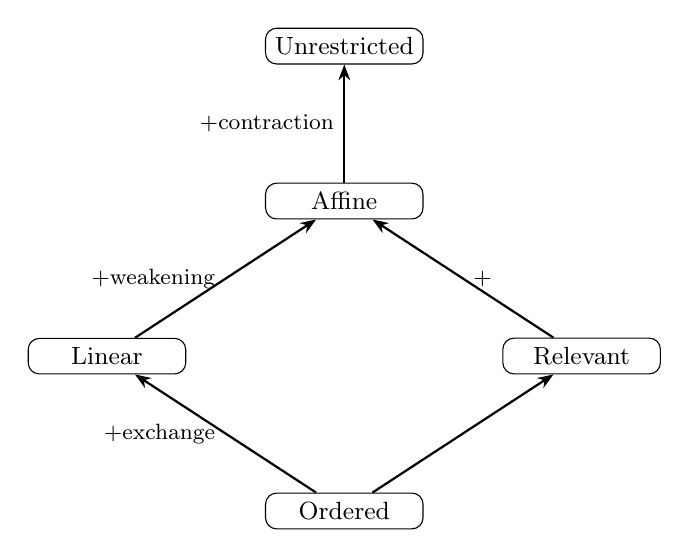
\begin{tikzpicture}[
  node distance=2cm,
  mod/.style={draw, rounded corners, minimum width=2cm,
    text centered, font=\small},
  arr/.style={-{Stealth[length=2mm]}, thick}
]
  \node[mod] (ord) {Ordered};
  \node[mod, above left=1.5cm and 1cm of ord] (lin) {Linear};
  \node[mod, above right=1.5cm and 1cm of ord] (rel) {Relevant};
  \node[mod, above left=1.5cm and 1cm of rel] (aff) {Affine};
  \node[mod, above=1.5cm of aff] (un) {Unrestricted};

  \draw[arr] (ord) -- (lin) node[midway, left, font=\footnotesize] {+exchange};
  \draw[arr] (ord) -- (rel) node[midway, right, font=\footnotesize] {};
  \draw[arr] (lin) -- (aff) node[midway, left, font=\footnotesize] {+weakening};
  \draw[arr] (rel) -- (aff) node[midway, right, font=\footnotesize] {+};
  \draw[arr] (aff) -- (un) node[midway, left, font=\footnotesize] {+contraction};
\end{tikzpicture}
\end{center}

In \ephapax{}, the programmer works primarily in the affine and linear
nodes of this lattice. The refinement journey moves \emph{down} the
lattice (from affine to linear), adding conservation constraints.
Moving \emph{up} the lattice (from linear to affine to unrestricted)
adds degrees of freedom---but each degree of freedom has a cost, as
we have argued throughout this paper.

\end{document}
